\section{Data}

In this work, we utilize stellar data from Gaia Data Release 2 (DR2)~\cite{GAIADR2}.  
From the extensive Gaia catalog, we select only those stars 
for which radial velocities $v_{\text{rad}}$ were measured relative to the Sun via the Doppler effect.  
To manage the dataset size efficiently, we apply a random subsampling procedure, 
restricting the dataset to entries with a random index less than $10^8$.

For each selected star, we extract key parameters from Gaia DR2: 
parallax $p$ and its associated uncertainty $\sigma_{p}$, 
radial velocity $v_{\text{rad}}$ with measurement uncertainty $\sigma_{v}$, 
and Galactic coordinates — specifically, latitude $b$ and longitude $l$.

To focus our analysis on stars approximately lying in the Galactic plane, we apply a cut on the latitude, considering only stars with latitude $\vert b \vert < 5^\circ$.  
To ensure data quality, we retain only stars with a relative parallax uncertainty below 20\%, 
and a radial velocity uncertainty less than 5~\unit{\kilo\meter\per\second}.  

After applying these criteria, we obtain a sample of $\text{N}_{\text{stars}}=75\text{,}659$ stars. 
The upper panel of Figure~\ref{fig:DataModelPresentation} shows the distribution of their radial velocities with respect to the Sun, plotted as a function of their Galactic longitude. Only values within the range $[-200, 200]$~\unit{\kilo\meter\per\second} are displayed to improve the data readability, although the full dataset includes velocities extending up to approximately 500~\unit{\kilo\meter\per\second}. 
These extreme values are likely outliers, and a more refined data-cleaning procedure could further improve the quality of the analysis.

\begin{figure}[H]
    \centering
    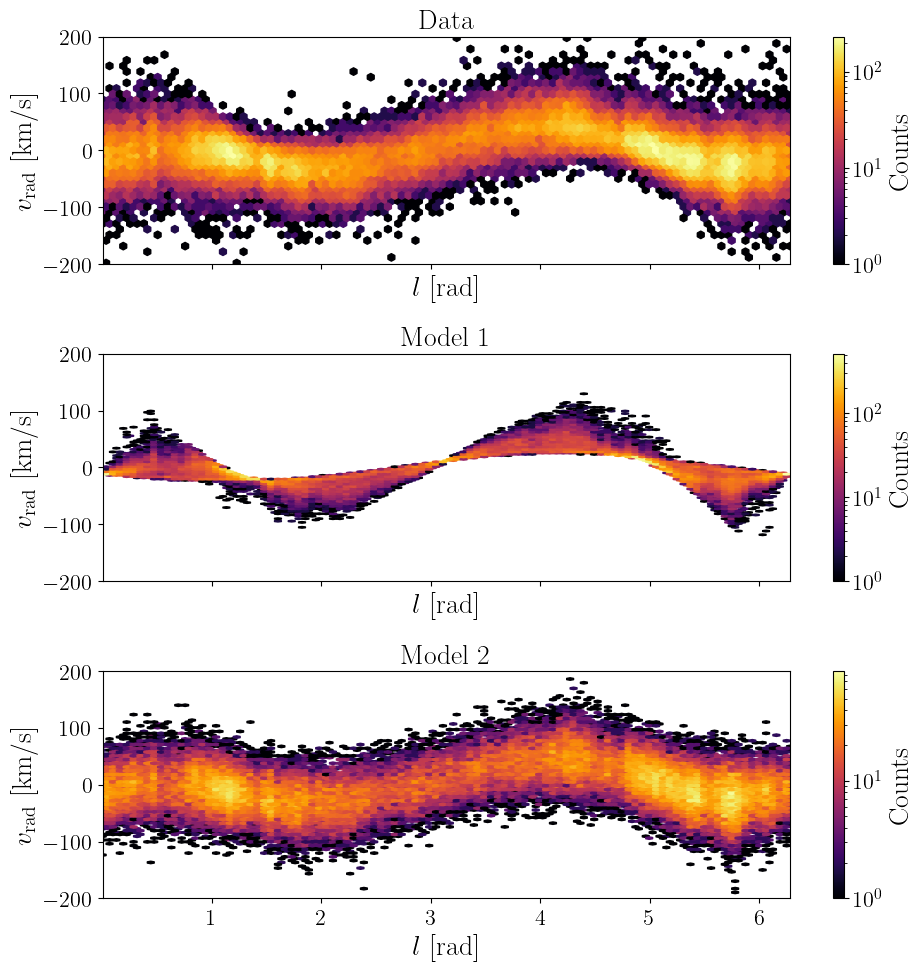
\includegraphics[width=0.95\columnwidth]{Fig/DataModelPresentation.png}
    \caption{Upper: observed radial velocities in the range $[-200, 200]$~\unit{\kilo\meter\per\second}. Middle: predicted radial velocities from the first model. Lower: simulated radial velocity distribution under the second model.}
    \label{fig:DataModelPresentation}
\end{figure}
